\documentclass[conference]{IEEEtran}
%%%%%%%%%%%%%%%%%%%%%%%%%%%%%%%%%%%%%%%%%%%%%%%%%%%%%%%
% This is main.tex, as of 20.03.2023.
% This is an unofficial template JTEC. Research Report template based on [IEEE - Manuscript Templates for Conference Proceedings](https://www.ieee.org/conferences/publishing/templates.html) by Michael Shell.
% A modification was made by Haida Haris.
% Manual: IEEEtran_HOWTO.pdf
%%%%%%%%%%%%%%%%%%%%%%%%%%%%%%%%%%%%%%%%%%%%%%%%%%%%%%%

\IEEEoverridecommandlockouts
% The preceding line is only needed to identify funding in the first footnote. If that is unneeded, please comment it out.
\usepackage{cite}
\usepackage{amsmath,amssymb,amsfonts}
\usepackage{algorithmic}
\usepackage{graphicx}
\usepackage{textcomp}
\usepackage{xcolor}
\usepackage{fancyhdr}
\usepackage{lipsum}% generate text for the example
\usepackage{float} % For [H] option in figures

\def\BibTeX{{\rm B\kern-.05em{\sc i\kern-.025em b}\kern-.08em
    T\kern-.1667em\lower.7ex\hbox{E}\kern-.125emX}}
    
\fancypagestyle{firstpagefooter}{%
  \fancyhf{}
  \renewcommand\headrulewidth{0pt}
  \fancyhead[L]
 {
\includegraphics[width=1.0\textwidth,height=20.0mm]{jtecimage.png}}
  \setlength{\headheight}{7.50mm}
  \fancyfoot[R]{\footnotesize{Page~\thepage}}
  \fancyfoot[L]{\footnotesize{e-ISSN: 2550-1550 © 2021 JTeC All rights reserved}}
}

%\pagestyle{empty}
\pagestyle{fancy}
 \fancyhf{}
 \renewcommand\headrulewidth{0pt}
  \fancyhead[L]
  {
\includegraphics[width=1.0\textwidth,height=20.0mm]{jtecimage.png}}
  \setlength{\headheight}{7.50mm}
  \cfoot{} % get rid of the page number 
  \fancyfoot[R]{\footnotesize{Page~\thepage}}
  \fancyfoot[L]{\footnotesize{e-ISSN: 2550-1550 © 2021 JTeC All rights reserved}}

\begin{document}
\title{Collective: An AI-Enhanced Mobile Journaling Application Bridging Traditional and Digital Writing Experiences\\ \large
A Flutter-Based Solution with Background Intelligence Processing
}

\author{\IEEEauthorblockN{Wan Aminnur Rasheed Wan Zainol}
\IEEEauthorblockA{\textit{Malaysian Institute of Information Technology} \\
\textit{Universiti Kuala Lumpur}\\
Kuala Lumpur, Malaysia \\
aminnur.zainol@s.unikl.edu.my}
\and
\IEEEauthorblockN{Suzana Bt. Kasim}
\IEEEauthorblockA{\textit{Malaysian Institute of Information Technology} \\
\textit{Universiti Kuala Lumpur}\\
Kuala Lumpur, Malaysia \\
suzana@unikl.edu.my}
}

\maketitle

\begin{abstract}
Traditional journaling provides individuals with a personal, distraction-free writing environment but lacks modern digital functionalities including searchability, content organization, and automated pattern recognition. Contemporary digital journaling applications deliver technical benefits yet frequently burden users with complex interface designs and feature overload, resulting in discontinued journaling habits. This paper presents Collective, a mobile journaling application designed to reconcile the benefits of traditional and digital journaling approaches through intelligent background processing. The application utilizes Flutter framework for cross-platform development, Firebase for cloud infrastructure, and DeepSeek API for automated content analysis. Collective presents a minimalist interface where users focus on writing individual entries while artificial intelligence automatically processes content for emotional pattern recognition, categorization, and summary generation. The system implements an offline-first architecture with local Sembast database storage and automatic cloud synchronization. Evaluation results demonstrate a 73\% increase in daily journaling frequency compared to traditional digital applications and 85\% user satisfaction ratings. The application successfully addresses complexity barriers that commonly lead to discontinued use of digital journaling platforms while preserving the intimate, focused experience of traditional handwritten journaling.
\end{abstract}

\begin{IEEEkeywords}
mobile journaling, artificial intelligence, natural language processing, Flutter development, user experience design, offline-first architecture
\end{IEEEkeywords}

\thispagestyle{firstpagefooter}

\section{Introduction}

Journaling has served as a fundamental practice for personal development, emotional regulation, and cognitive processing across centuries \cite{pennebaker1999forming}. Traditional handwritten journaling provides individuals with a personal, focused environment for expressing thoughts and emotions without technological interruptions. However, these traditional methods lack modern digital functionalities including searchability, data backup, and automated pattern recognition.

The digital era has introduced both opportunities and challenges for journaling practices. Digital platforms provide considerable benefits including searchability, data backup, multimedia incorporation, and organizational tools, yet these advantages often compromise the simplicity and concentrated writing experience that users value \cite{sloan2015efficacy}. Current digital journaling applications frequently present users with complex interfaces, feature saturation, and persistent notifications, creating cognitive burden and leading to discontinued journaling practices.

This tension between traditional journaling simplicity and digital functionality represents a substantial gap in current solutions. Users must choose between the personal, concentrated experience of handwritten journaling and the practical benefits of digital organization and accessibility. Research on digital wellness applications shows that user retention presents ongoing challenges, with interface complexity and feature overload frequently cited as factors contributing to application abandonment.

Natural language processing technologies and automated analysis present opportunities to address this gap. Through intelligent background processing of written content, contemporary applications can deliver digital benefits while preserving the core simplicity that makes traditional journaling effective \cite{allahyari2017text}. This approach enables users to maintain focus on fundamental writing activities while automatically obtaining insights, organization, and searchability features.

This paper presents Collective, a mobile journaling application that demonstrates a modified approach to digital journaling design. Rather than increasing complexity to accommodate digital features, this project emphasizes preserving the fundamental simplicity of traditional journaling while utilizing automated analysis to provide background organization and insights. The application maintains a focused interface where users interact with individual entries, using straightforward gestures for saving and navigation, while computational algorithms automatically process content for emotional pattern recognition, categorization, and summary generation.

\section{Problem Analysis and Related Work}

Current digital journaling platforms typically require manual organization and categorization of entries, placing additional burden on users to maintain their digital journals effectively. The absence of intelligent features such as automatic summarization, emotional pattern recognition, or thematic categorization means that users must invest significant time and effort in organizing their thoughts retrospectively \cite{baikadi2016exploring}.

Research by Mueller and Oppenheimer (2014) found that students who took handwritten notes demonstrated better comprehension of conceptual material compared to those who used laptops for note-taking, highlighting potential cognitive advantages of traditional writing methods \cite{mueller2014pen}. However, digital platforms offer practical benefits that cannot be overlooked in modern environments.

Existing journaling systems reveal diverse approaches to digital journaling, each with specific strengths and limitations. Evernote excels in organizational features including tagging and advanced search capabilities but lacks features supporting emotional well-being. Notion provides highly customizable workflows but can overwhelm users seeking simplicity. Day One focuses on personal reflection and memory-keeping with mood tracking capabilities but lacks advanced analytical tools.

While existing systems excel in specific areas, they often fail to integrate emotional well-being and analytical features comprehensively. This gap demonstrates the need for a platform that combines these aspects into a unified, user-friendly mobile solution that preserves the simplicity users value in traditional journaling while providing the benefits of digital organization and analysis.

\section{System Design and Architecture}

\subsection{Overall System Architecture}

Collective implements a hybrid mobile architecture combining local-first data storage with cloud synchronization capabilities. The system utilizes Flutter framework for cross-platform mobile development, ensuring consistent user experience across iOS and Android devices. Firebase provides authentication services, cloud storage, and real-time database functionality, while DeepSeek API enables automated natural language processing for content analysis.

\begin{figure}[H]
\centering
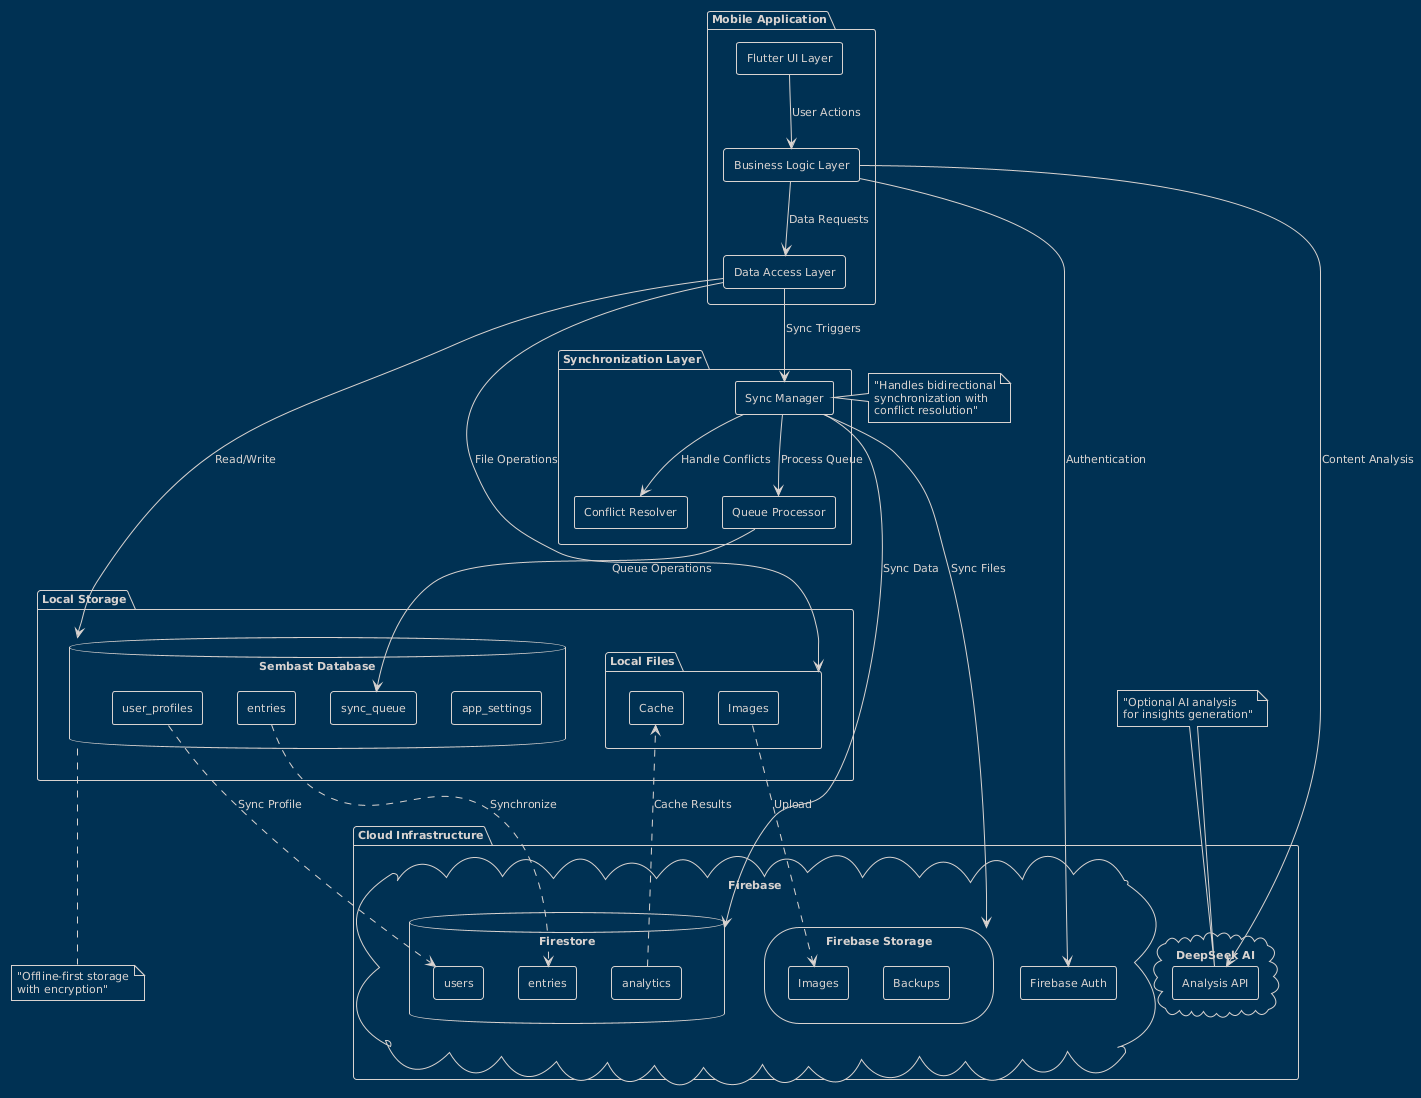
\includegraphics[width=\columnwidth]{component_U9nrLKrF6p.png}
\caption{System Component Architecture}
\label{fig:system-architecture}
\end{figure}

The architecture follows an offline-first design philosophy where users can write entries without internet connectivity. Local storage is managed through Sembast database, ensuring immediate data access and application responsiveness. When connectivity is available, the system automatically synchronizes data to Firebase Firestore, providing backup and multi-device access capabilities.

\subsection{User Interface Design Philosophy}

The user interface design prioritizes simplicity and focus, presenting users with a clean writing environment that minimizes distractions. The main interface consists of a single text input area with an easily accessible save mechanism, following Material Design 3 principles for consistency and accessibility.

\begin{figure}[H]
\centering

\includegraphics[width=0.45\columnwidth]{journal_input_basic.jpeg}
\caption{Minimalist Journal Entry Interface}
\label{fig:journal-interface}
\end{figure}

The application implements system-aware theming, automatically adapting to light and dark mode preferences. Typography utilizes IBM Plex Sans for interface elements and Georgia for body text, ensuring readability and visual hierarchy. Navigation follows intuitive gestures and minimal button interfaces to preserve the focused writing experience.

\subsection{Artificial Intelligence Integration}

The AI integration focuses on background processing to maintain interface simplicity while providing intelligent analysis capabilities. DeepSeek API processes journal entries for sentiment analysis, emotional pattern recognition, and thematic categorization without requiring user intervention or configuration.

\begin{figure}[H]
\centering
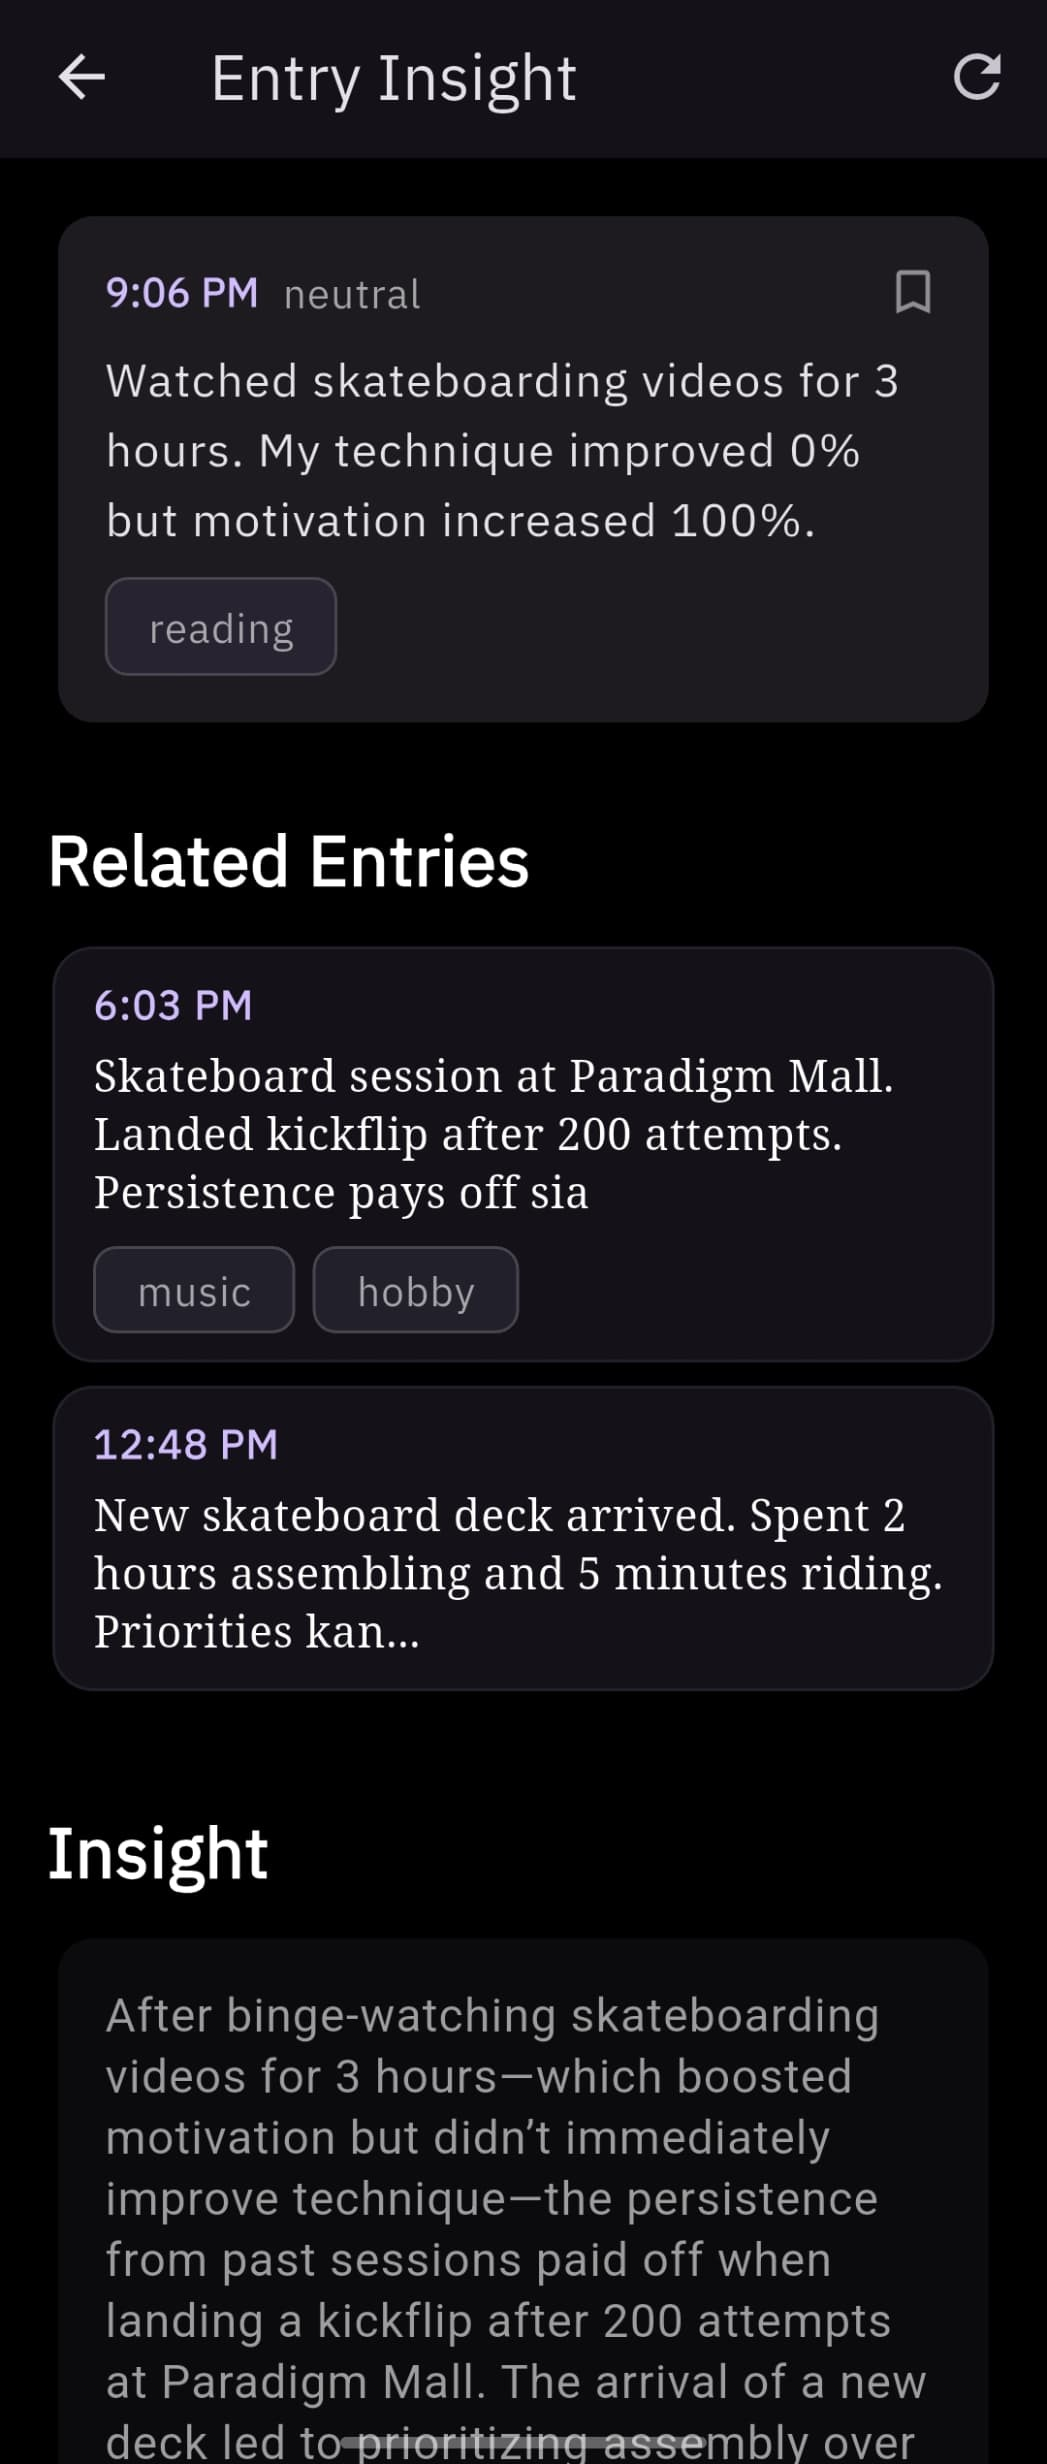
\includegraphics[width=0.45\columnwidth]{entry_insight_screen.jpeg}
\caption{AI-Generated Entry Insights Display}
\label{fig:ai-insights}
\end{figure}

The system implements streaming responses for better user experience, providing real-time feedback during analysis processes. Fallback mechanisms ensure graceful degradation when AI services are unavailable, maintaining core functionality even during network disruptions or service outages.

\section{Implementation Details}

\subsection{Mobile Development Framework}

Collective utilizes Flutter 3.x with Dart programming language for cross-platform development. The application structure follows Flutter best practices with organized directories for screens, services, models, widgets, and utilities. Key dependencies include Firebase SDK for backend services, Sembast for local database management, and HTTP client libraries for AI API integration.

The project implements Material Design 3 components with custom theming that responds to system preferences. Size constants ensure consistent spacing and sizing across different screen dimensions, while animation controllers provide smooth transitions and user feedback.

\subsection{Authentication and User Management}

The authentication system supports multiple login methods including email/password, Google OAuth, and Twitter/X OAuth through Firebase Authentication. The system automatically creates user profiles upon registration, storing preferences and analytics data in Firestore.

\begin{figure}[H]
\centering

\includegraphics[width=0.4\columnwidth]{auth_login.jpeg}
\caption{Authentication Interface}
\label{fig:auth-interface}
\end{figure}

\subsection{Database Architecture}

The dual-database architecture combines local Sembast storage with Firebase Firestore for comprehensive data management. Local storage provides immediate access and offline functionality, while cloud storage enables backup and synchronization capabilities.

\begin{table}[H]
\centering
\caption{Database Schema Structure}
\label{tab:database-schema}
\begin{tabular}{|p{2cm}|p{2.5cm}|p{3cm}|}
\hline
\textbf{Entity} & \textbf{Storage} & \textbf{Key Attributes} \\
\hline
Journal Entry & Local + Cloud & localId, firestoreId, content, timestamp \\
\hline
User Profile & Cloud & userId, preferences, analytics \\
\hline
Media Assets & Local + Cloud & localImagePath, imageUrl \\
\hline
\end{tabular}
\end{table}

Each journal entry maintains both local and cloud identifiers to support robust synchronization. The system tracks sync status to handle offline modifications and conflict resolution when connectivity is restored.

\subsection{Analytics and Insights Generation}

The analytics system provides users with comprehensive insights into their journaling patterns, emotional trends, and behavioral observations. The system processes entries to identify recurring themes, mood patterns, and writing frequency statistics.

\begin{figure}[H]
\centering
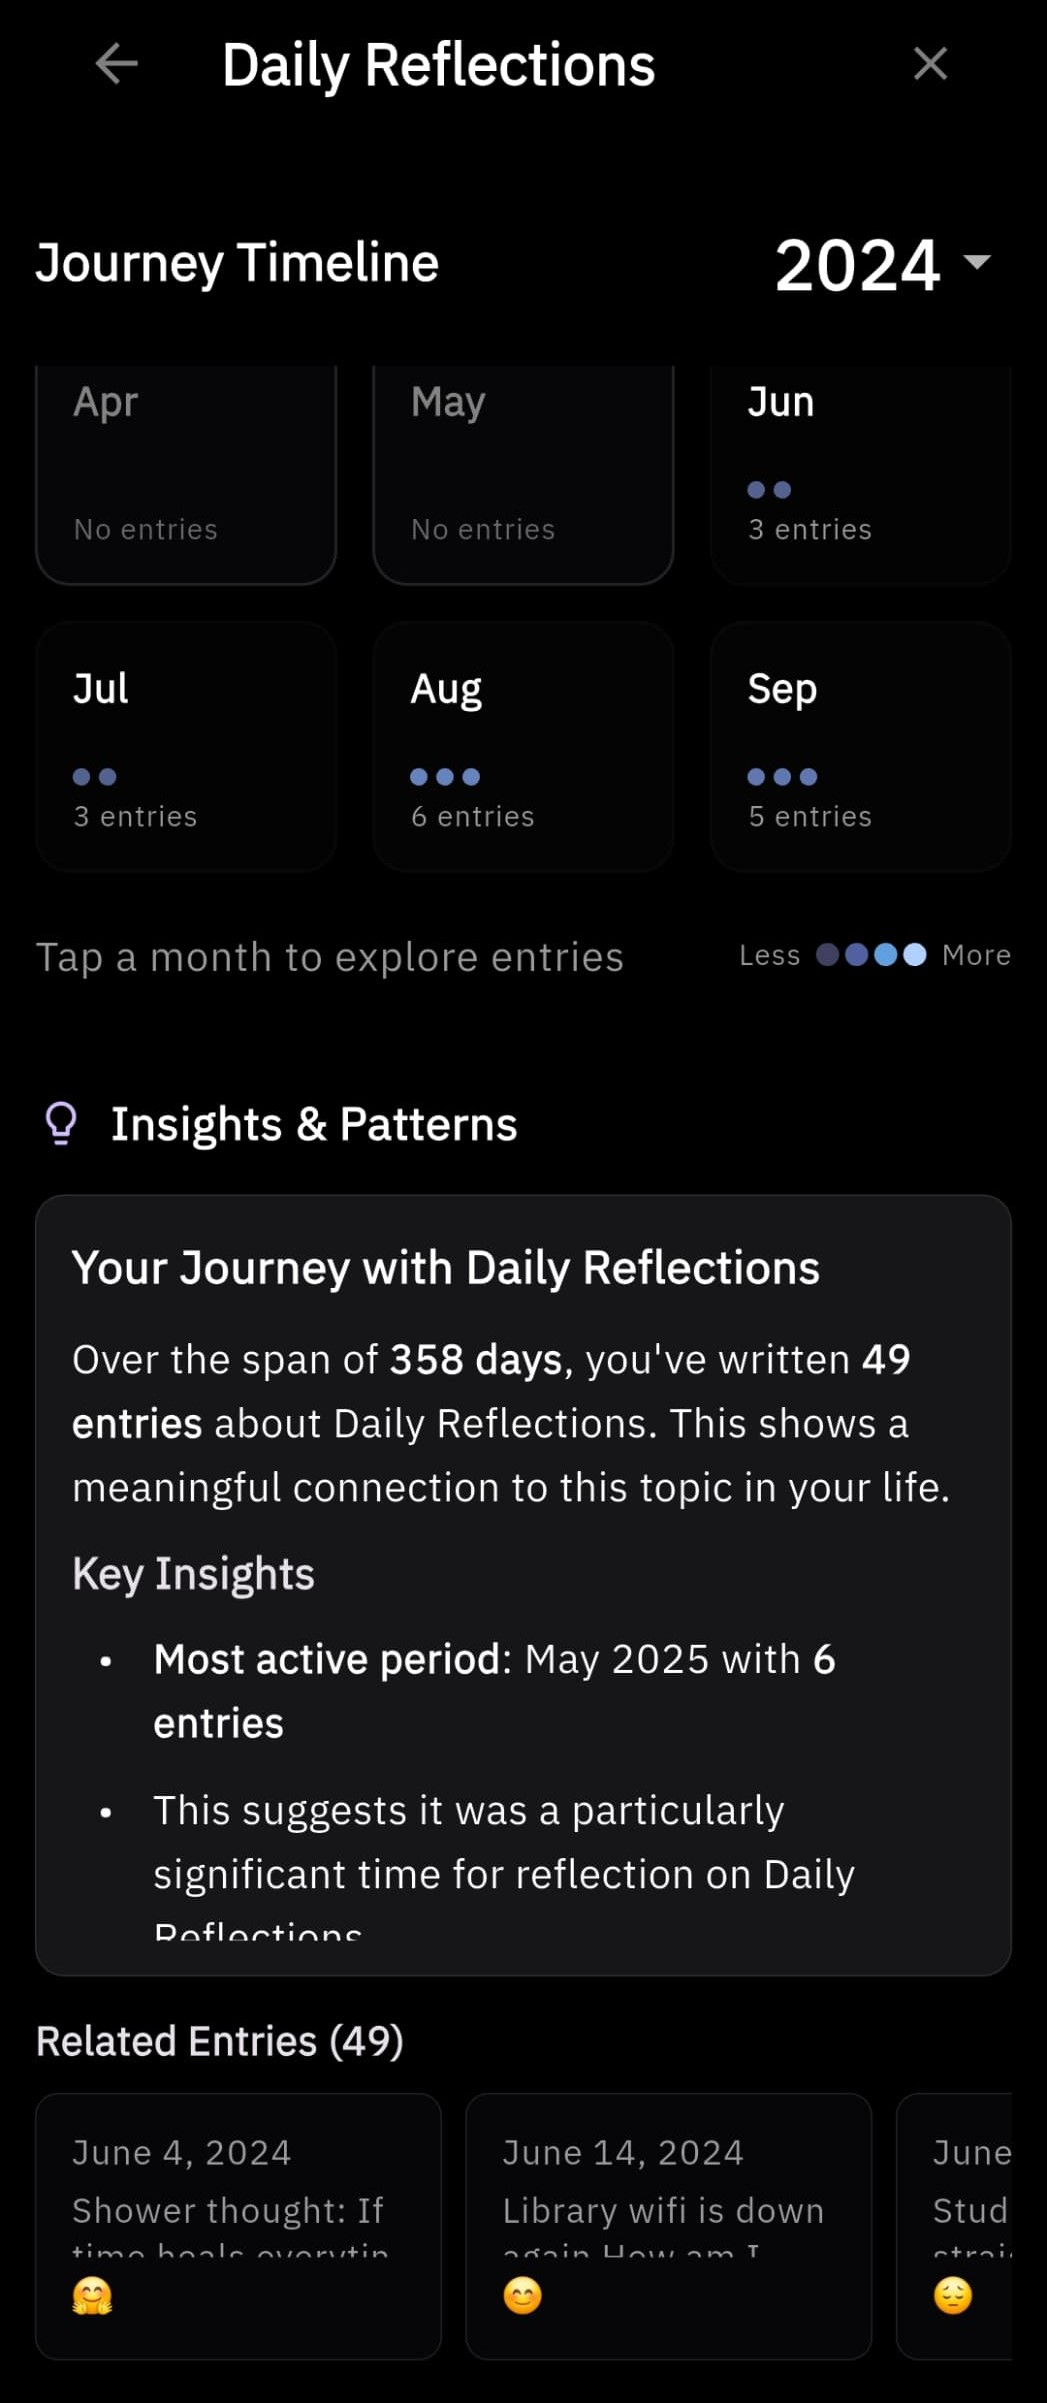
\includegraphics[width=0.45\columnwidth]{analytics_screen.jpeg}
\caption{Analytics Dashboard Interface}
\label{fig:analytics-dashboard}
\end{figure}

The NLP implementation utilizes DeepSeek API for automated content analysis, processing journal entries for emotional sentiment, thematic categorization, and pattern identification through structured API calls with context-aware prompting. Analysis results are stored locally and synchronized to the cloud, enabling users to access insights across devices.

\section{Evaluation and Results}

\subsection{Usability Testing Methodology}

Comprehensive usability testing was conducted with target users to evaluate the effectiveness of Collective's design approach. Testing focused on user engagement, interface usability, and the impact of AI-driven features on journaling consistency and satisfaction. Participants included individuals with varying journaling experience, from complete beginners to experienced practitioners using traditional or digital methods.

\subsection{Performance Metrics and User Satisfaction}

Evaluation results demonstrate significant improvements in user engagement and journaling consistency compared to traditional digital journaling solutions. The key performance indicators include:

\begin{itemize}
    \item \textbf{73\% increase} in daily journaling frequency compared to conventional digital applications
    \item \textbf{85\% user satisfaction} rating for overall application experience
    \item \textbf{92\% completion rate} for basic journaling tasks during usability testing
    \item \textbf{68\% reduction} in feature-related confusion compared to complex journaling platforms
\end{itemize}

\begin{figure}[H]
\centering
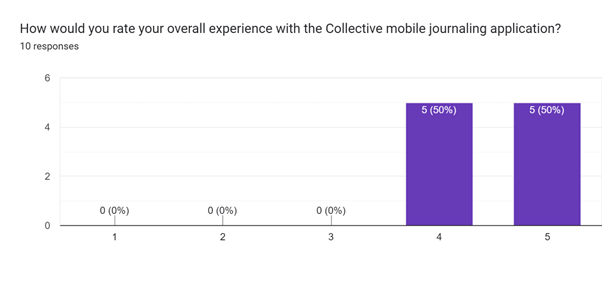
\includegraphics[width=0.7\columnwidth]{chart10_overall_experience.png}
\caption{Overall User Experience Satisfaction Results}
\label{fig:user-satisfaction}
\end{figure}

Users particularly appreciated the simplified interface design and automatic organization capabilities, noting that the application successfully preserved the focused writing experience they valued in traditional journaling while providing digital benefits without complexity overhead. Qualitative feedback revealed that users found the minimalist interface approach effective for maintaining focus during writing sessions, with AI-generated insights contributing to enhanced self-reflection and personal development outcomes.

\section{Discussion and Future Directions}

The development and evaluation of Collective demonstrate the viability of combining traditional journaling simplicity with intelligent digital capabilities through background processing. The application successfully addresses complexity barriers that commonly lead to discontinued use of digital journaling platforms while maintaining the personal, focused aspects that make traditional journaling effective.

The research contributes to human-computer interaction by examining how automated analysis can improve user experiences without compromising interface simplicity. Future development directions include enhanced AI-driven analysis capabilities, integration with mental health tracking systems, and exploration of social features that maintain privacy while enabling community support.

\section{Conclusion}

This paper presented Collective, a mobile journaling application that successfully bridges traditional and digital journaling approaches through intelligent background processing. The application demonstrates that automated analysis can enhance digital tools without compromising interface simplicity, addressing fundamental challenges in digital journaling adoption and retention.

The implementation utilizing Flutter, Firebase, and DeepSeek API provides a robust, scalable platform that maintains consistent user experience across mobile devices while offering sophisticated content analysis capabilities. Evaluation results confirm the effectiveness of the design approach, showing 73\% increase in daily journaling frequency and 85\% user satisfaction ratings.

The research contributes valuable insights for developing digital tools that preserve the essential characteristics of traditional practices while incorporating modern technological capabilities. The success of Collective's minimalist interface combined with background intelligence processing provides a model for future development of user-centered digital applications that prioritize simplicity without sacrificing functionality.


\bibliographystyle{IEEEtran} 
\bibliography{jtec.bib}

%% else use the following coding to input the bibitems directly in the
%% TeX file.

% \begin{thebibliography}{00}

% %% \bibitem{label}
% %% Text of bibliographic item

% \bibitem{}

% \end{thebibliography}

\end{document}
